\documentclass[twoside]{report}

\usepackage[landscape,inner=2cm,outer=12cm,marginparwidth=9cm,
            marginparsep=1.0cm,bottom=2cm]{geometry}

\setlength{\parskip}{1.1em}
\setlength{\parindent}{0em}
\usepackage{pdfpages}
\usepackage{amsmath}
\usepackage{amsfonts}
\usepackage{amssymb}
\usepackage{bigdelim}
\usepackage[usenames,dvipsnames]{pstricks}
\usepackage{booktabs}
\usepackage[T1]{fontenc}
\usepackage{listings}
\usepackage[T1]{fontenc}
\usepackage[utf8]{inputenc}
\usepackage{float}
\usepackage{graphicx}
\usepackage{cite}
\usepackage{hyperref}
\usepackage{layout}
\usepackage{titlesec}
\usepackage{fancyhdr}
\usepackage{pgf}
\usepackage{amsmath}
\usepackage{titlesec}
\usepackage{verbatim}
\usepackage{color}
\usepackage[font=small,labelfont=bf]{caption}
\usepackage{marginnote}
\usepackage{afterpage}
\usepackage[light,math]{iwona}
\usepackage{sectsty}

% No number sections
\renewcommand{\thesection}{}
\renewcommand{\thesubsection}{\arabic{section}.\arabic{subsection}}
\makeatletter
\def\@seccntformat#1{\csname #1ignore\expandafter\endcsname\csname the#1\endcsname\quad}
\let\sectionignore\@gobbletwo
\let\latex@numberline\numberline
\def\numberline#1{\if\relax#1\relax\else\latex@numberline{#1}\fi}
\makeatother

%Colors
\definecolor{purplefront}{RGB}{154,34,119}
\definecolor{purplesec}{RGB}{144,24,109}

%Define commands
\newcommand{\marginquote}[1]{\marginpar{\textcolor{gray}{\large\itshape\fontfamily{ppl}\selectfont#1}}}

% Paragraphs have proper breaks
\titlespacing\section{0pt}{12pt plus 4pt minus 2pt}{0pt plus 2pt minus 2pt}
\titlespacing\subsection{0pt}{12pt plus 4pt minus 2pt}{0pt plus 2pt minus 2pt}
\titlespacing\subsubsection{0pt}{12pt plus 4pt minus 2pt}{0pt plus 2pt minus 2pt}
\renewcommand{\figurename}{{\textbf{Image}}}
\sectionfont{\color{purplefront}}

%Fancyheader
\pagestyle{fancy}
\fancyheadoffset[leh,roh]{10cm}
\fancyhf{}
\fancyhead[LE,RO]{\textcolor{gray}{\thepage}}
\fancyhead[RE,LO]{\textcolor{gray}{\textsc{Fundamentals of Artificial Intelligence (57205HT16): Assignment 2 -
Happy, Sad, Mischievous or Mad?}}}
\renewcommand{\headrulewidth}{0pt}


\begin{document}
\begin{titlepage}
  \vspace{12cm}
	\raggedright
  {\Large \textbf{Interactivity in smart environments}\\}
  {\small\color{gray} Marc Coquand, Linus Lagerhjelm, Mattias Cederberg and Simon
  Asp\\}
  {\small\color{gray} Supervised by Helena}\\
  {\small\color{gray} Umeå University\\}

	\vfill

% Bottom of the page
	{\large \today\par}
\end{titlepage}

\renewcommand{\baselinestretch}{1.0}

\newpage

\pagecolor{purplefront}\afterpage{\nopagecolor}\thispagestyle{empty}
\marginpar{\textcolor{white}{\small{Assignment
1}\vspace{11cm}\\\large\textbf{Abstract
normally in form of a title}\\ {\small The
evening of Saturday, August 27th, 2011, the volunteer fire department in
Prattsville, New York held its annual clambake. The event has not historically
been associated with temperance, but that year, the festivities broke up early.
Prattsville is a sleepy town of fewer than 1,000 residents in the northern
Catskill Mountains, about 100 miles inland from the Atlantic Ocean. It’s
leaf-peeping country, not tropical storm country. But a hurricane was moving up
the East Coast, and Sunday’s forecast called for rain. Meteorologists had
predicted that the Catskills would get a peripheral spray, rather than the
storm’s brunt, which was slated for New York City and Long Island. Still, Tom
Olson, who was then fire chief, intended to be ready. }}} \newpage

\tableofcontents
\thispagestyle{empty}
\newpage

\section{Introduction}




The evening of
Saturday, August 27th, 2011, the volunteer fire department in Prattsville, New
York held its annual clambake. The event has not historically been associated
with temperance, but that year, the festivities broke up early. Prattsville is a
sleepy town of fewer than 1,000 residents in the northern Catskill Mountains,
about 100 miles inland from the Atlantic Ocean. It’s leaf-peeping country, not
tropical storm country. But a hurricane was moving up the East Coast, and
Sunday’s forecast called for rain. Meteorologists had predicted that the
Catskills would get a peripheral spray, rather than the storm’s brunt, which
was slated for New York City and Long Island. Still, Tom Olson, who was then
fire chief, intended to be ready.

\marginpar{ \captionof{figure}{This is a margin figure.}
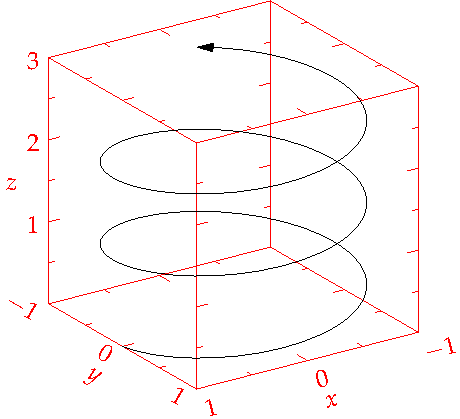
\includegraphics[width=\marginparwidth]{graphics/helix.pdf}} 

In his late 40s, with an average build and short, dark hair flecked with gray,
Olson has lived in Prattsville all his life. Soft-spoken almost to the point of
shyness, he delivers mail for a living, and cannot help but know most everyone
in town. Until 2011 Olson primarily associated flooding with cold weather. When
he was young, the Schoharie Creek — a gentle tributary of the Mohawk River that
runs along Main Street, past the firehouse — used to jam with ice, forcing
water onto the road. On such occasions, the fire department had often helped
pump out waterlogged basements. He suspected that Sunday might be similar.

\marginquote{``This is a very insipirational quote right here. Very
quoteworthy if I may say so myself.''}

Olson woke around 6:30AM at his home in the hills above town. He got in his
Dodge Ram 3500 pickup, a 2006 model that would not survive the day, and drove
down to the station, where he monitored the creek. Rain fell hard and warm
through the humid air. Though he felt no panic, at 8AM, he decided to man the
firehouse, sounding its alarm to summon to duty roughly 15 firefighters. As they
arrived, he sent them on foot in crews of three and four to knock on the doors
of homes he considered likely to flood. It might be wise, he thought, to suggest
to people living in low-lying areas that they take shelter at the firehouse.

\end{document}
